\documentclass[convert]{standalone}

\usepackage{marvosym}
\usepackage{tikz}

\begin{document}
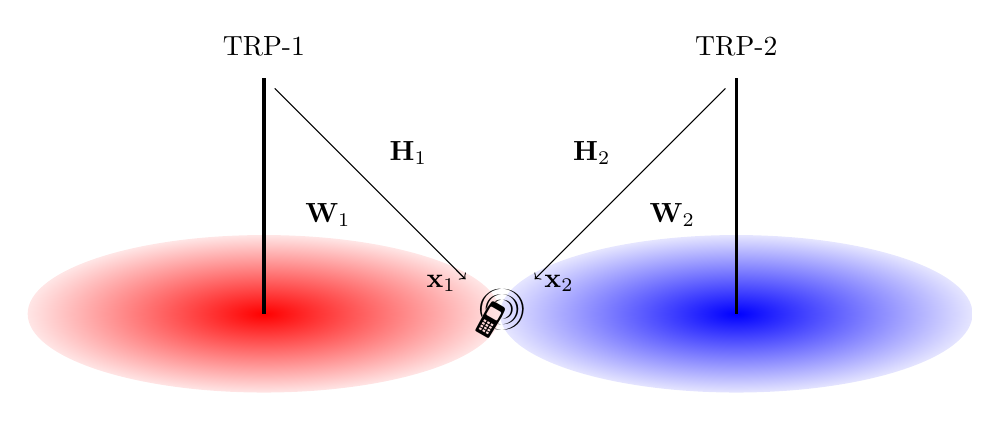
\begin{tikzpicture}
  \shade[inner color = red, outer color = red!10](-3, 0)ellipse(3 and 1);
  \shade[inner color = blue, outer color = blue!10](3, 0)ellipse(3 and 1);
  \draw [very thick](-3, 0) -> (-3, 3) node[label=90:TRP-1](trp1){};
  \draw [very thick](3, 0) -> (3, 3) node[label=90:TRP-2](trp2){};
  \node at (0, 0)[label=160:$\mathbf{x}_1$, label=20:$\mathbf{x}_2$](ue){\huge\Mobilefone};
  \draw (trp1) edge[->]node[label=45:$\mathbf{H}_1$, label=-135:$\mathbf{W}_1$]{} (ue);
  \draw (trp2) edge[->]node[label=135:$\mathbf{H}_2$, label=-45:$\mathbf{W}_2$]{} (ue);
\end{tikzpicture}
\end{document}

%%% Local Variables:
%%% mode: latex
%%% TeX-master: t
%%% End:
